\documentclass[12pt]{article}
\usepackage[T1]{fontenc}
\usepackage[utf8]{inputenc}
\usepackage{polski}
\usepackage{minted}
\usepackage{geometry}
\usepackage{natbib}
\usepackage{enumitem}
\usepackage{graphicx}
\usepackage{bold-extra}
\usepackage[font=small,labelfont=bf]{caption}
\usepackage{hyperref}
\usepackage{titlesec}
\usepackage{indentfirst}
\hyphenpenalty=10000
\tolerance=1000 \emergencystretch=2em
\titlelabel{\thetitle.\quad}

 \geometry{
     left=23mm,
     top=25mm,
     right=23mm
 }


\def\mydate{\leavevmode\hbox{\twodigits\day.\twodigits\month.\the\year}}
\def\twodigits#1{\ifnum#1<10 0\fi\the#1}

\begin{document}
%titlepage
\thispagestyle{empty}
\begin{center}
\begin{minipage}{0.75\linewidth}
    \centering
    
\includegraphics[width=0.45\linewidth]{agh_logo2.png}
    \par
    \vspace{2cm}
    {\bfseries{\scshape{\Huge  Teoria współbieżności}}}
    \par
    \vspace{1.7cm}
    {\scshape{\Large Laboratorium 11}}
    \par
    \vspace{0.8cm}
    {\scshape{\Large Teoria śladów}}
    \par
    \vspace{3cm}

    {\scshape{\Large Albert Gierlach}}\par
    \vspace{1cm}

    {\Large \mydate}
\end{minipage}
\end{center}
\clearpage



\section{Zadanie}
Dane są:

\begin{itemize}
    \item Alfabet A, w którym każda litera oznacza akcję.
    \item Relacja niezależności I, oznaczająca które akcje są niezależne (przemienne, tzn. można je wykonać w dowolnej kolejności i nie zmienia to wyniku końcowego).
    \item Słowo w oznaczające przykładowe wykonanie sekwencji akcji.
\end{itemize}


Napisz program w dowolnym języku, który:
\begin{enumerate}
    \item Wyznacza relację zależności D
    \item Wyznacza ślad [w] względem relacji I
    \item Wyznacza postać normalną Foaty FNF([w]) śladu [w]
    \item Wyznacza graf zależności dla słowa w
    \item Wyznacza postać normalną Foaty na podstawie grafu
\end{enumerate}

\section{Rozwiązanie}
Rozwiązanie powyższych zadań zostało wykonane przy użyciu języka Python. Użyte bilbioteki to: \emph{matplotlib}, \emph{numpy}, \emph{networkx}, \emph{network\_line\_graph}, \emph{graphviz}
W kodzie zostały dodane komentarze objaśniające poszczególne funkcje i metody.

\begin{minted}[frame=lines,
                framesep=2mm
                ]{python}
import os
import matplotlib.pyplot as plt
import numpy as np
import network_line_graph as nlg

from collections import defaultdict
from itertools import product
from pathlib import Path
from PIL import Image
from graphviz import Source


OUTPUT_FOLDER = "./output"


# Klasa przechowująca graf zależności.
# Reprezentacja grafu to lista sąsiedztwa
class Graph:
    def __init__(self, word, independent_operations):
        self.edges = defaultdict(list)
        self.word = word
        self.N = len(word)
        self.independency_rel = independent_operations
        self.node_labels = {i: k for i, k in enumerate(self.word)}
        self.build_edges()

    # zbuduj graf zależności dla danego słowa
    def build_edges(self):
        for pair in self.independency_rel.copy():
            self.independency_rel.add((pair[1], pair[0]))

        for i, l in enumerate(self.word[:-1]):
            edges_found = list(filter(lambda x: x[0] == l, self.independency_rel))
            for j, l2 in enumerate(self.word[i + 1:], i + 1):
                if not any([l2 == e for _, e in edges_found]):
                    self.edges[i].append(j)

    # rysuje półokrągłe strzałki z jednego węzła do innych
    def build_one_stage(self, letter_idx, d):
        a1 = np.zeros((self.N, self.N), dtype=bool)
        for e in self.edges[letter_idx]:
            a1[letter_idx, e] = True

        w1 = np.full((self.N, self.N), 0.6)
        w1[~a1] = np.nan

        if not np.all(np.isnan(w1)):
            nlg.draw(w1,
                     arc_above=d,
                     node_labels=self.node_labels,
                     node_order=np.array(range(self.N))
                     )

    # rysuj graf zależności
    # dla kazdego węzła rysuj odpowiednie krawędzie do innych węzłów
    def draw(self, dirs=None):
        if not dirs:
            dirs = [(v + 1) % 2 for v in range(self.N - 1)]

        for i, d in enumerate(dirs):
            self.build_one_stage(i, d)

    # usuwa krawędzie przechodnie
    def remove_transitive_edges(self):
        to_remove = set()
        for i in range(self.N):
            for j in self.edges[i]:
                for k in list(set(self.edges[i]) & set(self.edges[j])):
                    to_remove.add((i, k))

        self.remove_edges(list(to_remove))

    def remove_edges(self, to_remove):
        for a, b in to_remove:
            self.edges[a].remove(b)

    # zapisz graf do pliku .png
    def save_graph(self, fname):
        self.draw()
        self.save_graph_and_crop(fname, [-2, 2])

    def save_graph_and_crop(self, fname, lims=None):
        fname = f"{OUTPUT_FOLDER}/{fname}.png"
        ax = plt.gca()
        ax.set_ylim(lims)
        plt.savefig(fname, bbox_inches='tight')
        plt.clf()

        self.crop_white_space(fname)

    # przycina obrazek tak, aby zredukować białe ramki wokół obrazu
    def crop_white_space(self, fname):
        im = Image.open(fname)
        pix = np.asarray(im)
        pix = pix[:, :, 0:3]
        idx = np.where(pix - 255)[0:2]
        box = list(map(min, idx))[::-1] + list(map(max, idx))[::-1]
        region_pix = np.asarray(im.crop(box))
        im = Image.fromarray(region_pix)
        im.save(fname)

    # konwertuj graf do postaci DOT oraz wygeneruj plik .png z grafem
    def to_dot_format(self):
        output_string = ["digraph g{"]

        for k, e_list in self.edges.items():
            for v in e_list:
                output_string.append(f"\t{k} -> {v}")

        for k, label in self.node_labels.items():
            output_string.append(f"\t{k}[label={label}]")

        output_string.append("}")

        fname = f"{OUTPUT_FOLDER}/{self.word}_dot.txt"
        with open(fname, "wt") as f:
            f.write('\n'.join(output_string))

        g = Source.from_file(filename=fname)
        g.render(format='png')
        os.rename(f"{fname}.png", f"{OUTPUT_FOLDER}/{self.word}_dot.png")

    # wyznacz postać normalną na podstawie grafu
    # Algorytm:
    # 1) Znajdź wierzchołki, do których nie wchodzi żadna krawędź
    # 2) Ze znalezionych wierzchołków stwórz klasę Foaty
    # 3) Usuń znalezione wierzchołki oraz krawędzie z nich wychodzące
    # 4) Powtarzaj kroki 1-3 dopóki graf istnieje
    def to_foata(self):
        foata_normal = []
        in_degrees = {k: 0 for k in self.edges.keys()}
        for edge_list in self.edges.values():
            for e in edge_list:
                in_degrees[e] += 1

        while len(in_degrees):
            tops = []
            for k, v in in_degrees.items():
                if v == 0:
                    tops.append(k)

            for letter in tops:
                for edge in self.edges[letter]:
                    in_degrees[edge] -= 1

                del in_degrees[letter]

            foata_normal.append(''.join(sorted(map(self.node_labels.get, tops))))

        return foata_normal


class Problem:
    def __init__(self, alphabet, word, independency_relation):
        self.alphabet = alphabet
        self.word = word
        self.dependency_rel = None
        self.independency_rel = independency_relation
        self.independency_rel |= {(b, a) for a, b in self.independency_rel}  # symmetry

    # wyznacz relacje zależności
    # 1) Wygeneruj wszystkie możliwe pary z liter alfabetu
    # 2) Usuń wszystkie pary, które są w relacji niezależności
    def calculate_dependency_relation(self):
        return set(product(list(self.alphabet), repeat=2)) - self.independency_rel

    # wyznacza ślad słowa
    # 1) stwórz pusty zbiór wygenerowanych słów i dodaj do niego początkowe słowo
    # 2) dla każdego słowa ze zbioru zamieniaj pozycjami sąsiednie litery w słowie
    #    jeśli są w relacji niezależności
    # 3) każde nowo dodane słowo dodaj do zbioru wynikowego
    # 4) powtarzaj kroki 2-3 dopóki są generowane nowe słowa
    def calculate_trace(self):
        word_set = {self.word}

        while True:
            next_set = set(word_set)
            for w in word_set:
                for i in range(len(w) - 1):
                    prev, c1, c2, rest = w[:i], w[i], w[i + 1], w[min(i + 2, len(w)):]
                    if (c1, c2) in self.independency_rel:
                        next_set.add(prev + c2 + c1 + rest)

            if word_set == next_set:
                break
            word_set = next_set

        return word_set

    # przekształca słowo do postaci normalnej Foaty
    # Algorytm:
    # 1) dla każdej litery alfabetu stwórz pusty stos
    # 2) dla każdej litery w słowie czytanym od prawej do lewej wykonaj:
    #    - dodaj literę (l1) na odpowiadający jej stos
    #    - dla każdej litery (l2) będącej w relacji zależności z rozważaną literą (l1)
    #      dodaj pusty znacznik na stos tej litery (l2)
    # 3) zdejmij wszystkie litery, które są na wierzchołkach stosu
    # 4) ze zdjętych liter utwórz klasę Foaty
    # 5) dla każdej zdjętej litery ściąg ze stosów odpowiadające im znaczniki
    # 6) powtarzaj 3-5 dopóki każdy stos nie jest pusty
    def foata_normal_form(self):
        stacks = defaultdict(list)
        for letter in reversed(self.word):
            stacks[letter].append(letter)
            for c in self.alphabet:
                if c != letter and (letter, c) in self.dependency_rel:
                    stacks[c].append(None)

        foata_normal = []
        while any([len(s) for s in stacks.values()]):
            tops = [s[-1] for s in stacks.values() if len(s) and s[-1] is not None]
            for letter in tops:
                stacks[letter].pop()
                for c in self.alphabet:
                    if c != letter and (letter, c) in self.dependency_rel:
                        stacks[c].pop()

            foata_normal.append(''.join(sorted(tops)))

        return foata_normal

    def generate_graph(self, fname):
        graph = Graph(self.word, self.independency_rel)
        graph.remove_transitive_edges()
        graph.save_graph(fname + "_reduced")
        return graph

    def solve(self):
        def tuple_to_str(t):
            return "(" + ', '.join(t) + ")"

        print("Relacja zależności I = ", end='')
        print(f"{{{', '.join(map(tuple_to_str, sorted(self.independency_rel)))}}}")

        self.dependency_rel = self.calculate_dependency_relation()
        print("Relacja zależności D = ", end='')
        print(f"{{{', '.join(map(tuple_to_str, sorted(self.dependency_rel)))}}}")

        print("Ślad [w] względem relacji I: ", end='')
        traces = self.calculate_trace()
        print('[' + ', '.join(sorted(traces)) + ']')

        print("Postać normalna Foaty śladu [w]: ", end='')
        foata_normal = self.foata_normal_form()
        print(''.join(map(lambda s: f"({s})", foata_normal)))

        print("Generowanie grafu zależności... ", end='')
        G = self.generate_graph(f"{self.word}_graph")
        print("wygenerowano")

        print("Postać normalna Foaty na podstawie grafu: ", end='')
        print(''.join(map(lambda s: f"({s})", G.to_foata())))

        print("Generowanie grafu w formacie DOT... ", end='')
        G.to_dot_format()
        print("wygenerowano")


if __name__ == '__main__':
    Path(OUTPUT_FOLDER).mkdir(exist_ok=True)

    Problem(
        {'a', 'b', 'c', 'd'},
        'baadcb',
        {('a', 'd'), ('b', 'c')}
    ).solve()

    Problem(
        {'a', 'b', 'c', 'd', 'e', 'f'},
        'acdcfbbe',
        {('a', 'd'), ('b', 'e'), ('c', 'd'), ('c', 'f')}
    ).solve()

\end{minted}
Wykonanie programu dało następujące wyniki:
\begin{minted}[frame=lines,
                framesep=2mm,
                breaklines
                ]{text}
Relacja zależności I = {(a, d), (b, c), (c, b), (d, a)}
Relacja zależności D = {(a, a), (a, b), (a, c), (b, a), (b, b), (b, d), (c, a), (c, c), (c, d), (d, b), (d, c), (d, d)}
Ślad [w] względem relacji I: [baadbc, baadcb, badabc, badacb, bdaabc, bdaacb]
Postać normalna Foaty śladu [w]: (b)(ad)(a)(bc)
Generowanie grafu zależności... wygenerowano
Postać normalna Foaty na podstawie grafu: (b)(ad)(a)(bc)
Generowanie grafu w formacie DOT... wygenerowano

Relacja zależności I = {(a, d), (b, e), (c, d), (c, f), (d, a), (d, c), (e, b), (f, c)}
Relacja zależności D = {(a, a), (a, b), (a, c), (a, e), (a, f), (b, a), (b, b), (b, c), (b, d), (b, f), (c, a), (c, b), (c, c), (c, e), (d, b), (d, d), (d, e), (d, f), (e, a), (e, c), (e, d), (e, e), (e, f), (f, a), (f, b), (f, d), (f, e), (f, f)}
Ślad [w] względem relacji I: [accdfbbe, accdfbeb, accdfebb, acdcfbbe, acdcfbeb, acdcfebb, acdfcbbe, acdfcbeb, acdfcebb, adccfbbe, adccfbeb, adccfebb, adcfcbbe, adcfcbeb, adcfcebb, adfccbbe, adfccbeb, adfccebb, daccfbbe, daccfbeb, daccfebb, dacfcbbe, dacfcbeb, dacfcebb, dafccbbe, dafccbeb, dafccebb]
Postać normalna Foaty śladu [w]: (ad)(cf)(c)(be)(b)
Generowanie grafu zależności... wygenerowano
Postać normalna Foaty na podstawie grafu: (ad)(cf)(c)(be)(b)
Generowanie grafu w formacie DOT... wygenerowano
\end{minted}
\vspace{0.5cm}

\begin{center}
\centering
    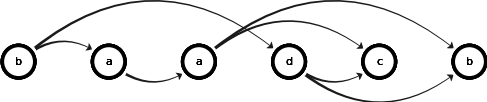
\includegraphics[scale=0.8]{baadcb_graph_reduced.png}
    \captionof{figure}{Zminimalizowany graf zależności słowa baadcb}
\end{center}

\newpage
\noindent
Graf słowa baadcb w formacie DOT:
\begin{minted}[frame=lines,
                framesep=2mm
                ]{text}
digraph g{
	0 -> 1
	0 -> 3
	1 -> 2
	2 -> 4
	2 -> 5
	3 -> 4
	3 -> 5
	0[label=b]
	1[label=a]
	2[label=a]
	3[label=d]
	4[label=c]
	5[label=b]
}
\end{minted}

\begin{center}
\centering
    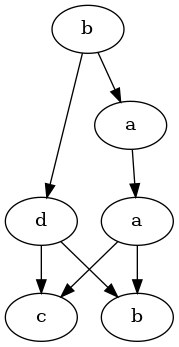
\includegraphics[scale=0.5]{baadcb_dot.png}
    \captionof{figure}{Zminimalizowany graf zależności słowa baadcb wygenerowany przy pomocy graphviz}
\end{center}

\vspace{0.5cm}

\begin{center}
\centering
    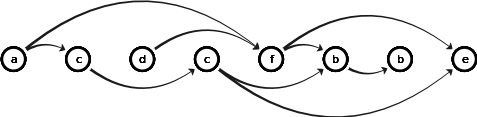
\includegraphics[scale=0.8]{acdcfbbe_graph_reduced.png}
    \captionof{figure}{Zminimalizowany graf zależności słowa acdcfbbe}
\end{center}

\noindent
Graf słowa acdcfbbe w formacie DOT:
\begin{minted}[frame=lines,
                framesep=2mm
                ]{text}
digraph g{
	0 -> 1
	0 -> 4
	1 -> 3
	2 -> 4
	3 -> 5
	3 -> 7
	4 -> 5
	4 -> 7
	5 -> 6
	0[label=a]
	1[label=c]
	2[label=d]
	3[label=c]
	4[label=f]
	5[label=b]
	6[label=b]
	7[label=e]
}
\end{minted}

\begin{center}
\centering
    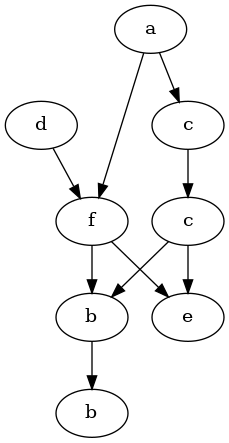
\includegraphics[scale=0.5]{acdcfbbe_dot.png}
    \captionof{figure}{Zminimalizowany graf zależności słowa acdcfbbe wygenerowany przy pomocy graphviz}
\end{center}

Przedstawione wyniki są poprawne i zgadzają się z ręcznie wyliczonymi wynikami z poprzednich laboratoriów.

\newpage
\section{Bibliografia}
\begin{itemize}
    \item \url{http://citeseerx.ist.psu.edu/viewdoc/download?doi=10.1.1.38.4401&rep=rep1&type=pdf}
    \item \url{https://en.wikipedia.org/wiki/Trace_theory}
    \item \url{https://en.wikipedia.org/wiki/DOT_(graph_description_language)}

\end{itemize}

\end{document}
